% T1 maps motion
\begin{figure}[ht]
    \centering
    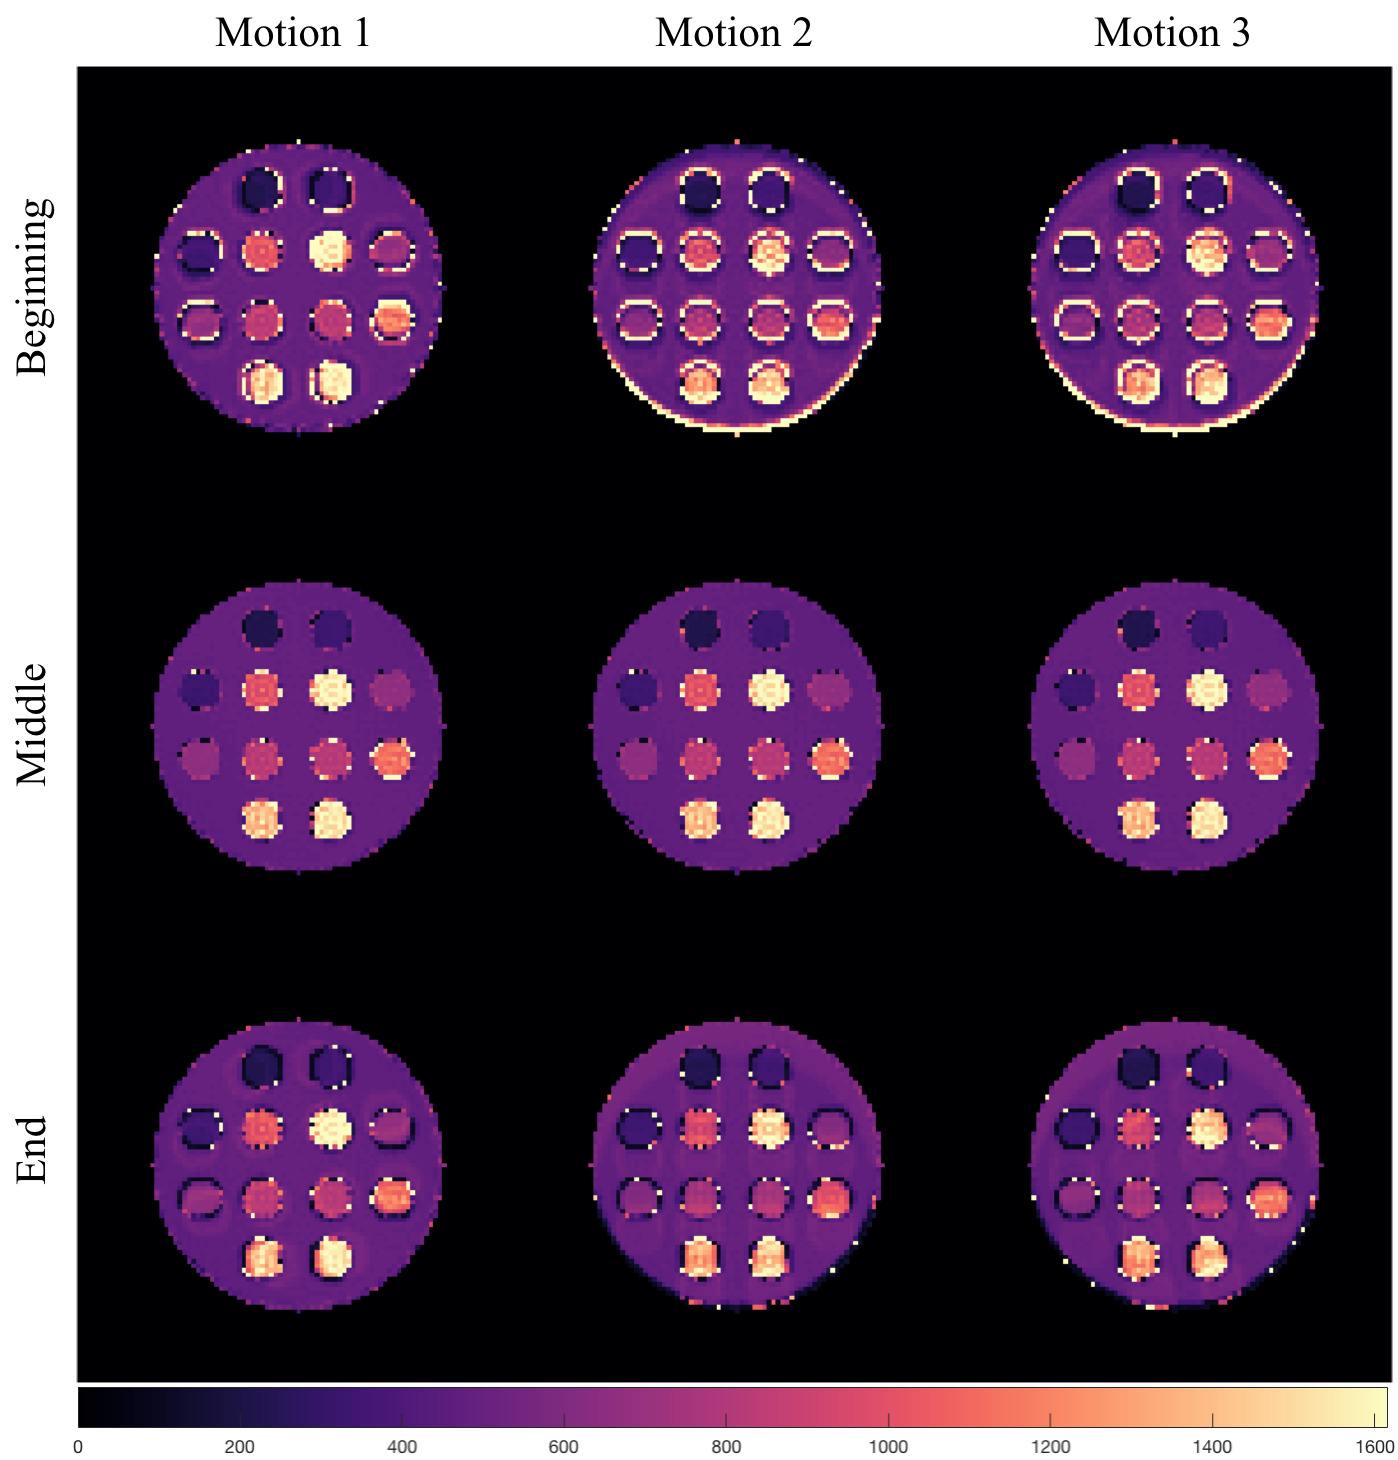
\includegraphics[width=1\textwidth]{images/mrf/T1mapsmotion}
    \caption{Motion corrupted $T_1$ quantitative maps for all 9 types of motion traces. First column corresponds to the \textit{motion 1} trace (continuous rotation about the z-axis), the second column corresponds to the \textit{motion 2} trace (continuous translation along the y-axis) and the third column corresponds to the \textit{motion 3} trace (continuous rotation about the z-axis and continuous translation along the y-axis). Different lines correspond to a different onset of motion.}
    \label{fig:appendixT1mapsmotion}
\end{figure}

% T1 maps differences motion
\begin{figure}[ht]
    \centering
    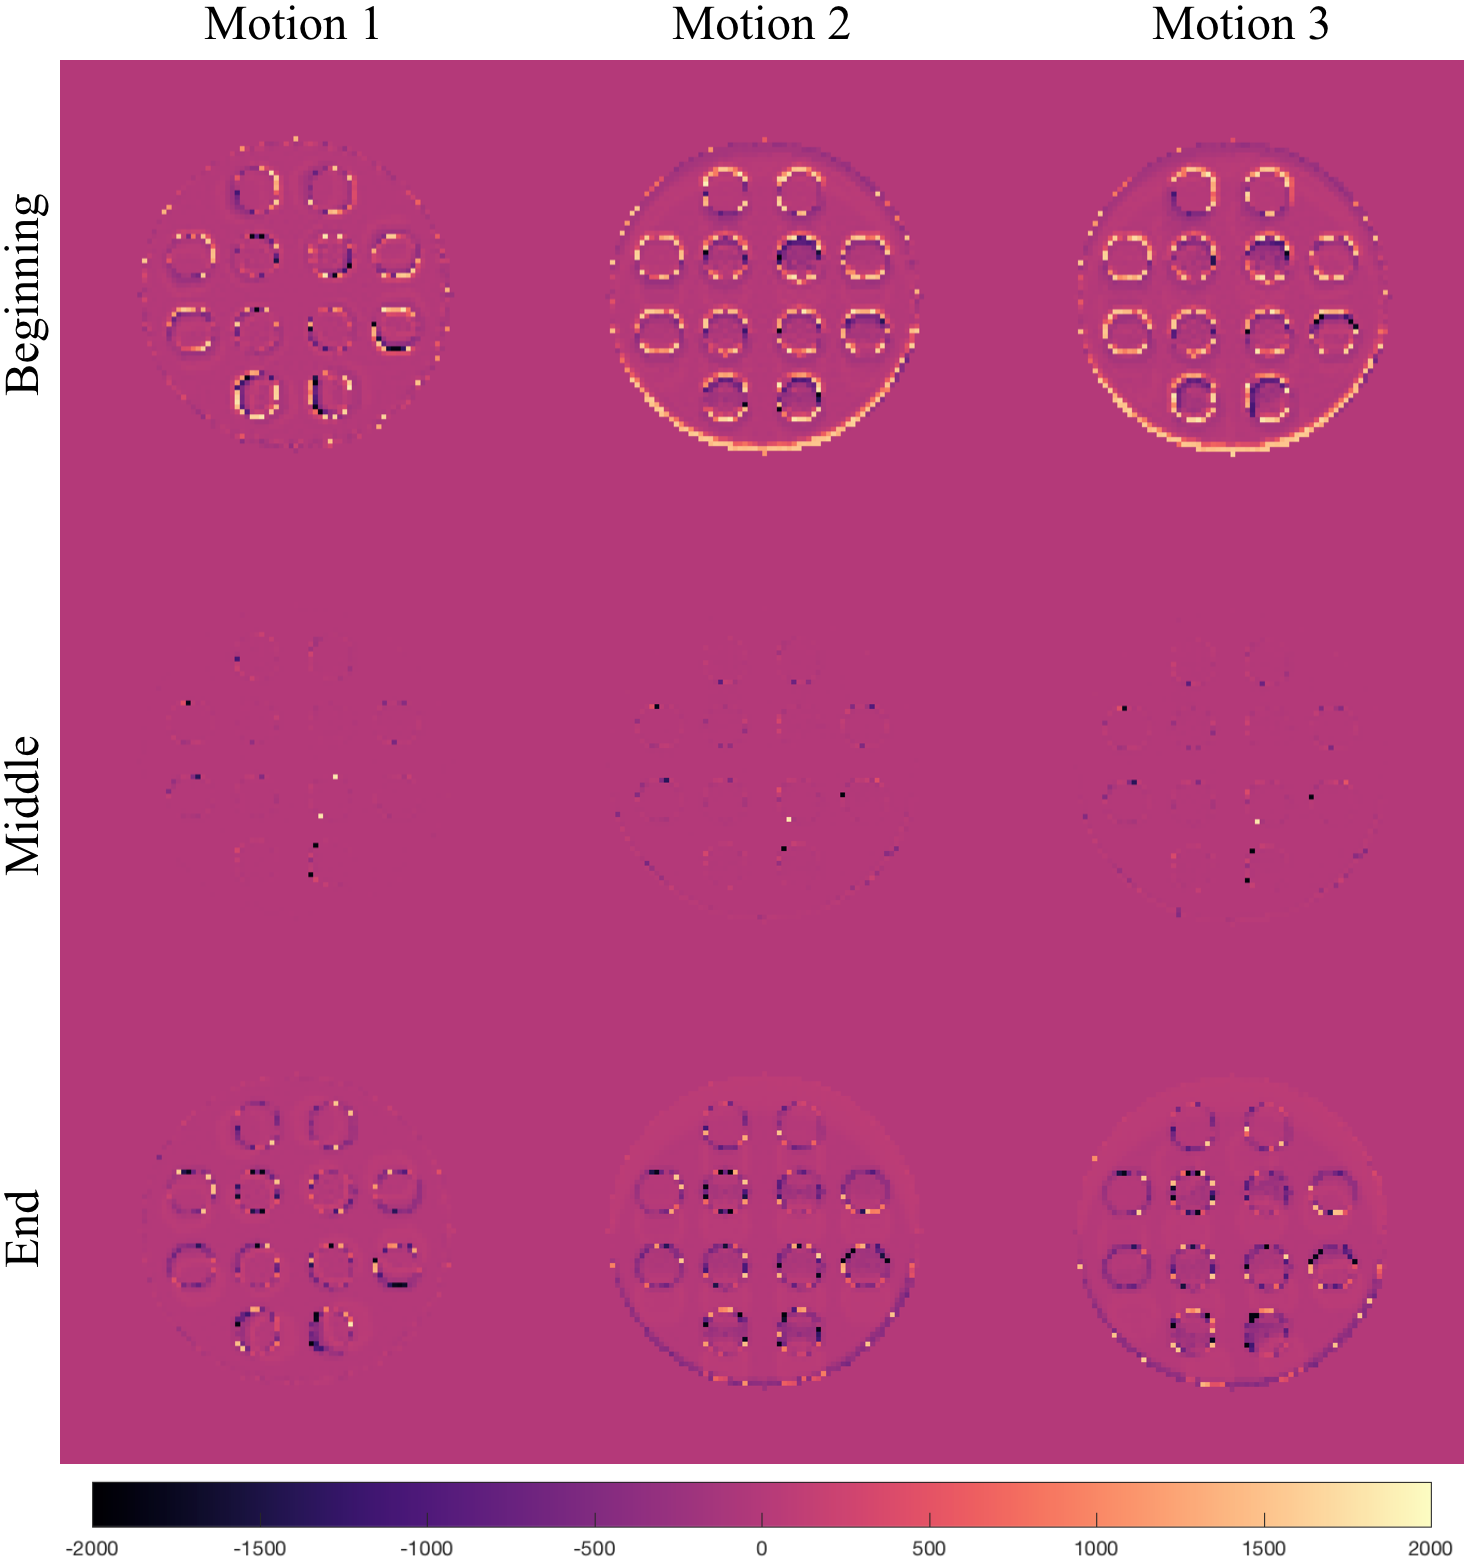
\includegraphics[width=1\textwidth]{images/mrf/T1SimuMinusT1Real}
    \caption{Difference between $T_1^{motion \, \, corrupted}$ and $T_1^{motion \, \, free}$ for all 9 types of motion traces. First column corresponds to the \textit{motion 1} trace (continuous rotation about the z-axis), the second column corresponds to the \textit{motion 2} trace (continuous translation along the y-axis) and the third column corresponds to the \textit{motion 3} trace (continuous rotation about the z-axis and continuous translation along the y-axis). Different lines correspond to a different onset of motion.}
    \label{fig:T1SimuMinusT1Real}
\end{figure}

% T2 maps motion
\begin{figure}[ht]
    \centering
    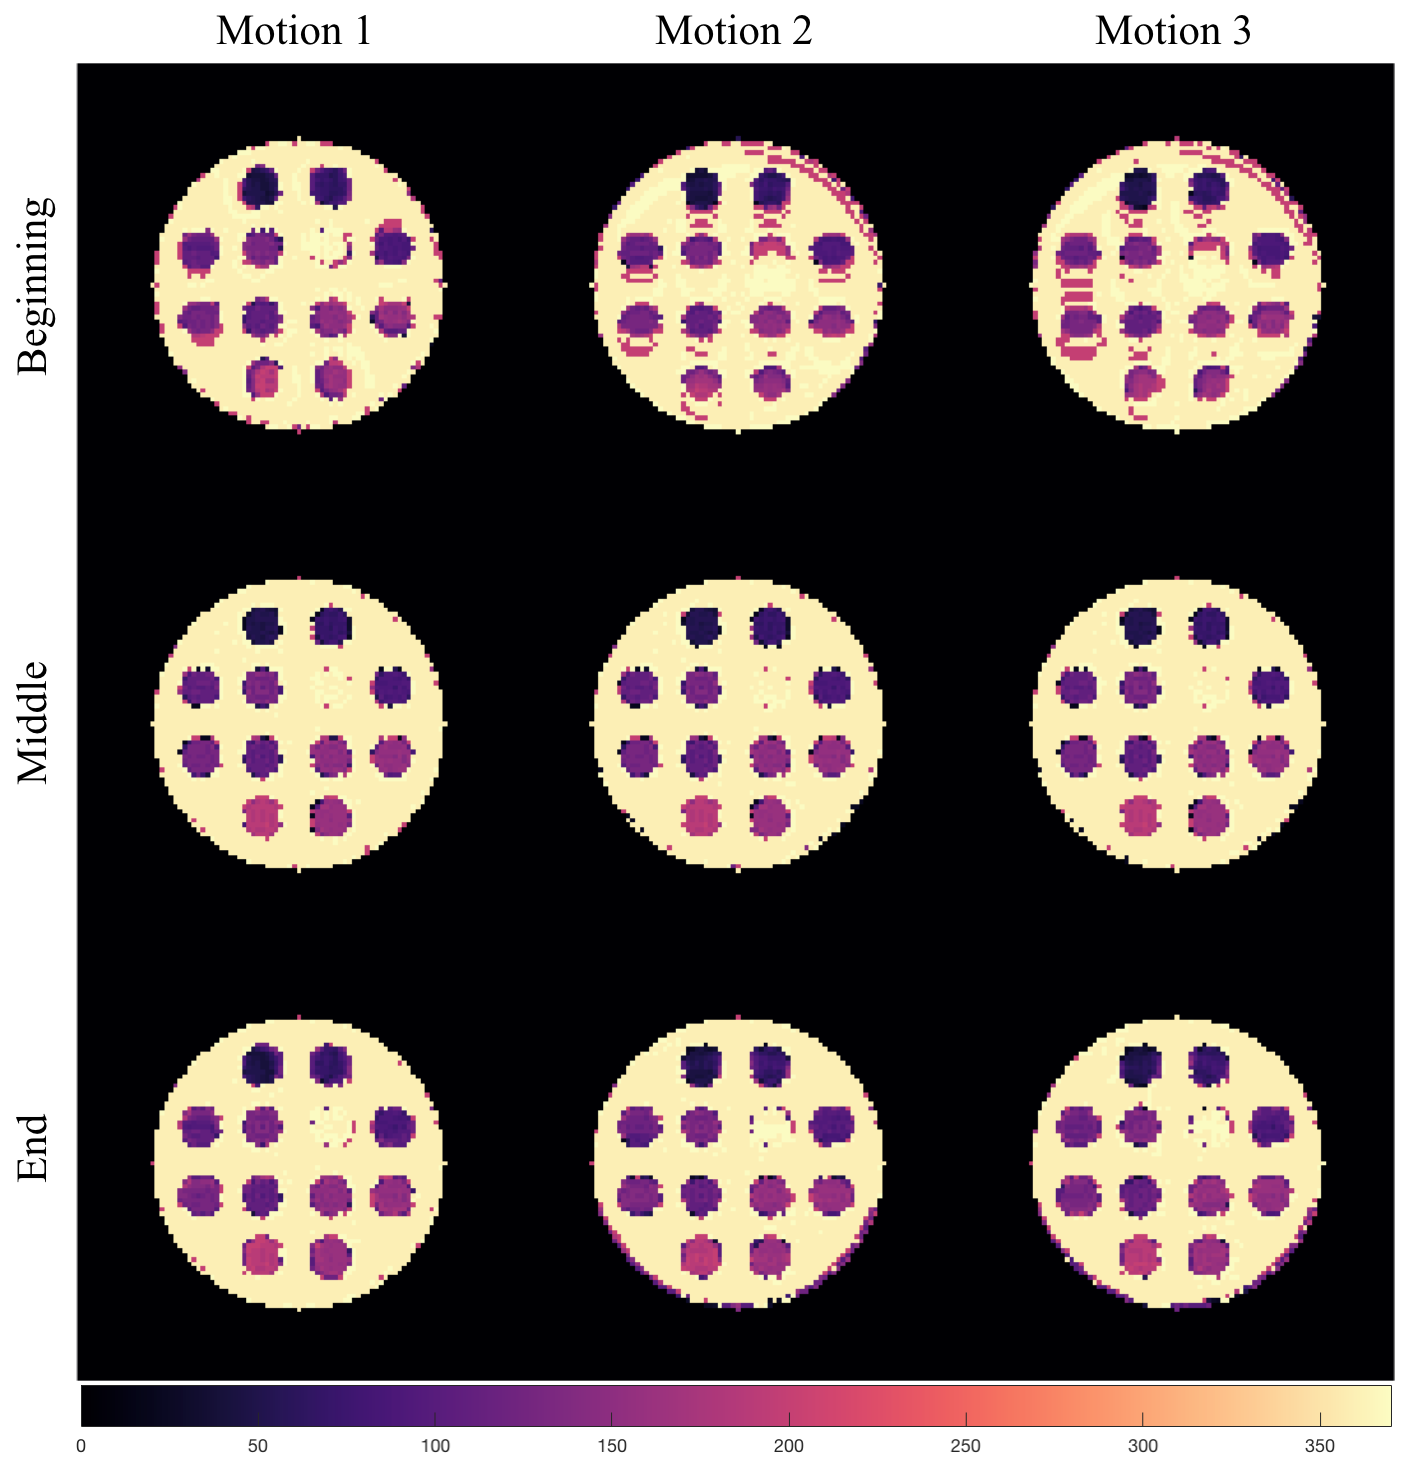
\includegraphics[width=1\textwidth]{images/mrf/T2mapsmotion}
    \caption{Motion corrupted $T_2$ quantitative maps for all 9 types of motion traces. First column corresponds to the \textit{motion 1} trace (continuous rotation about the z-axis), the second column corresponds to the \textit{motion 2} trace (continuous translation along the y-axis) and the third column corresponds to the \textit{motion 3} trace (continuous rotation about the z-axis and continuous translation along the y-axis). Different lines correspond to a different onset of motion.}
    \label{fig:appendixT2mapsmotion}
\end{figure}

% T2 maps differences motion
\begin{figure}[ht]
    \centering
    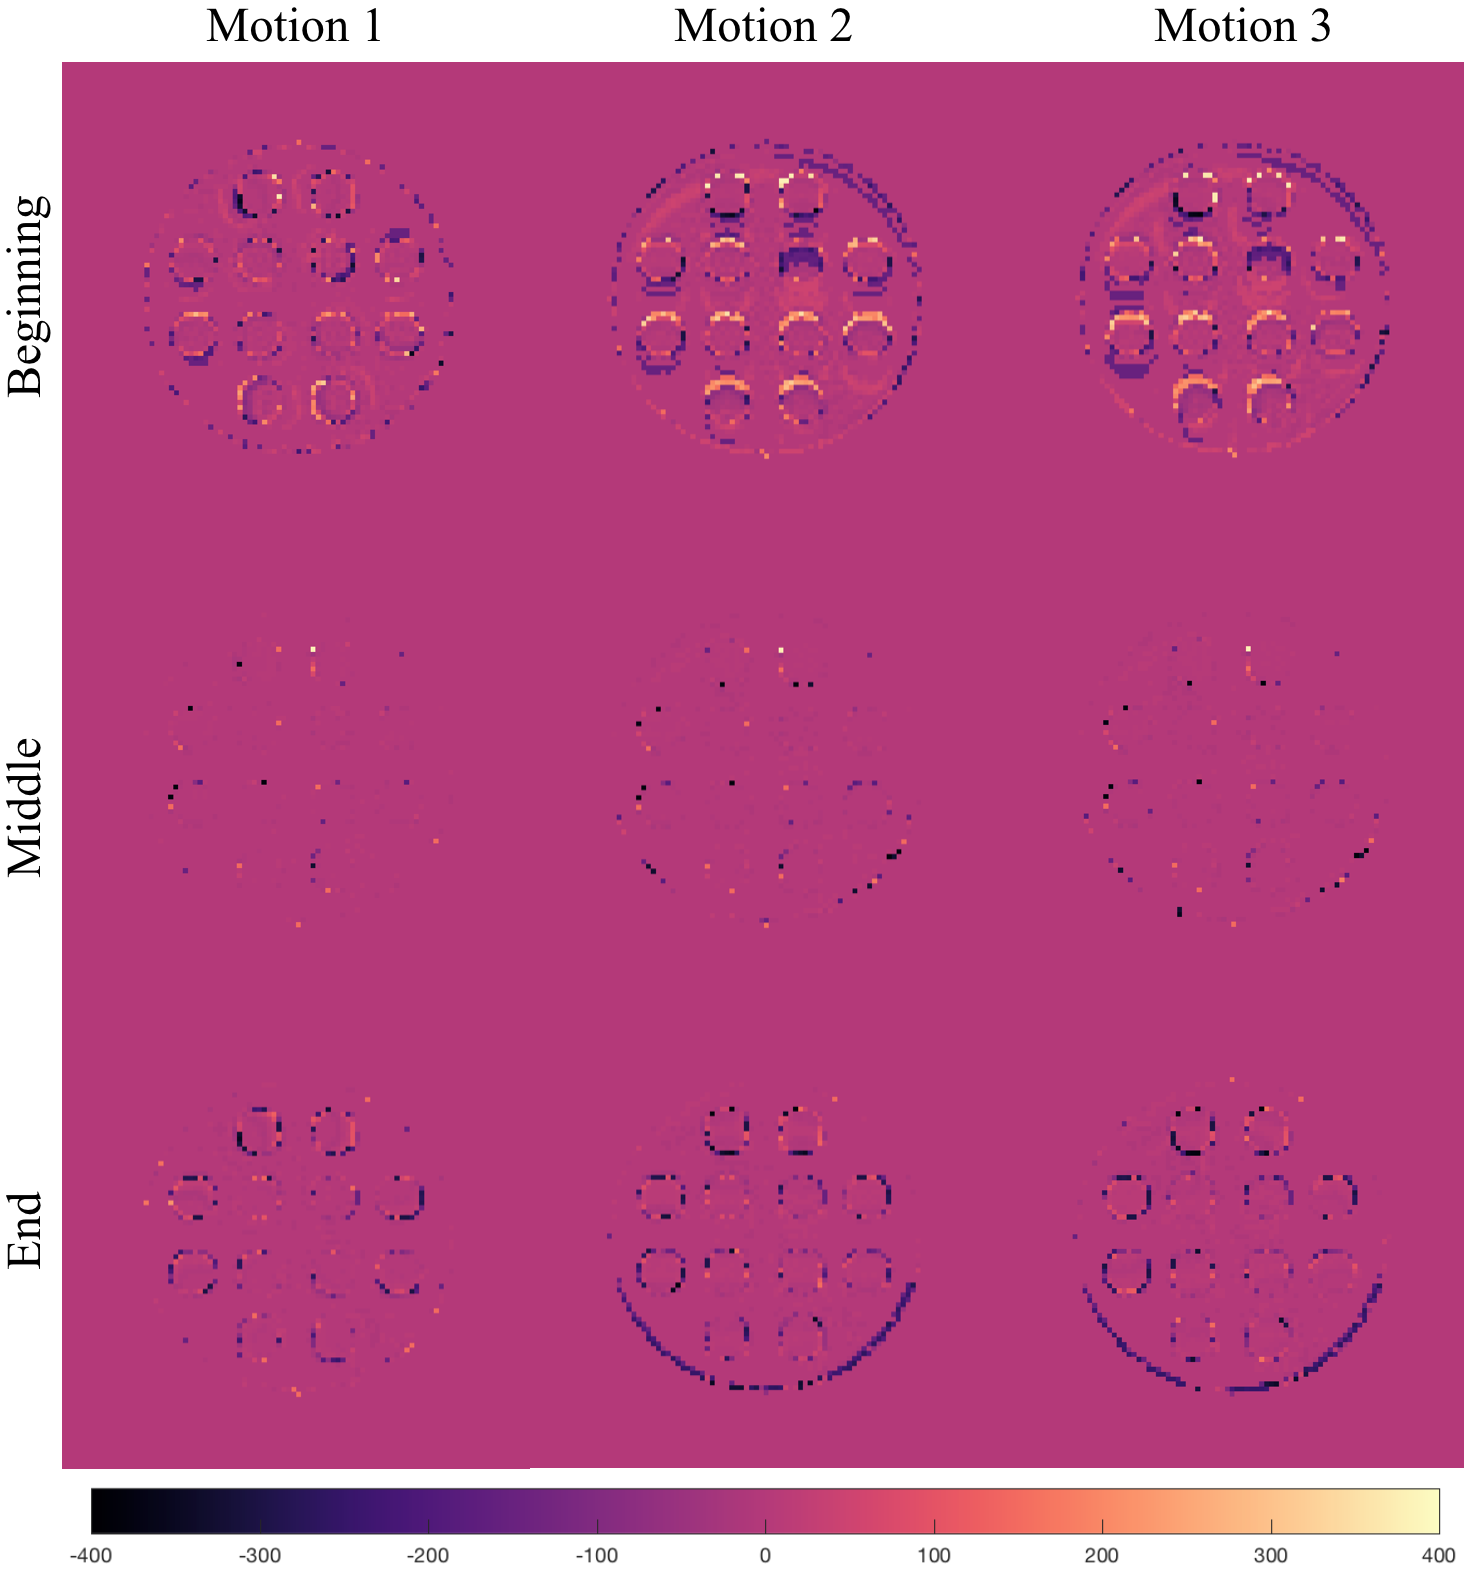
\includegraphics[width=1\textwidth]{images/mrf/T2SimuMinusT2Real}
    \caption{Difference between $T_2^{motion \, \, corrupted}$ and $T_2^{motion \, \, free}$ for all 9 types of motion traces. First column corresponds to the \textit{motion 1} trace (continuous rotation about the z-axis), the second column corresponds to the \textit{motion 2} trace (continuous translation along the y-axis) and the third column corresponds to the \textit{motion 3} trace (continuous rotation about the z-axis and continuous translation along the y-axis). Different lines correspond to a different onset of motion.}
    \label{fig:T2SimuMinusT2Real}
\end{figure}

% Score maps motion
\begin{figure}[ht]
    \centering
    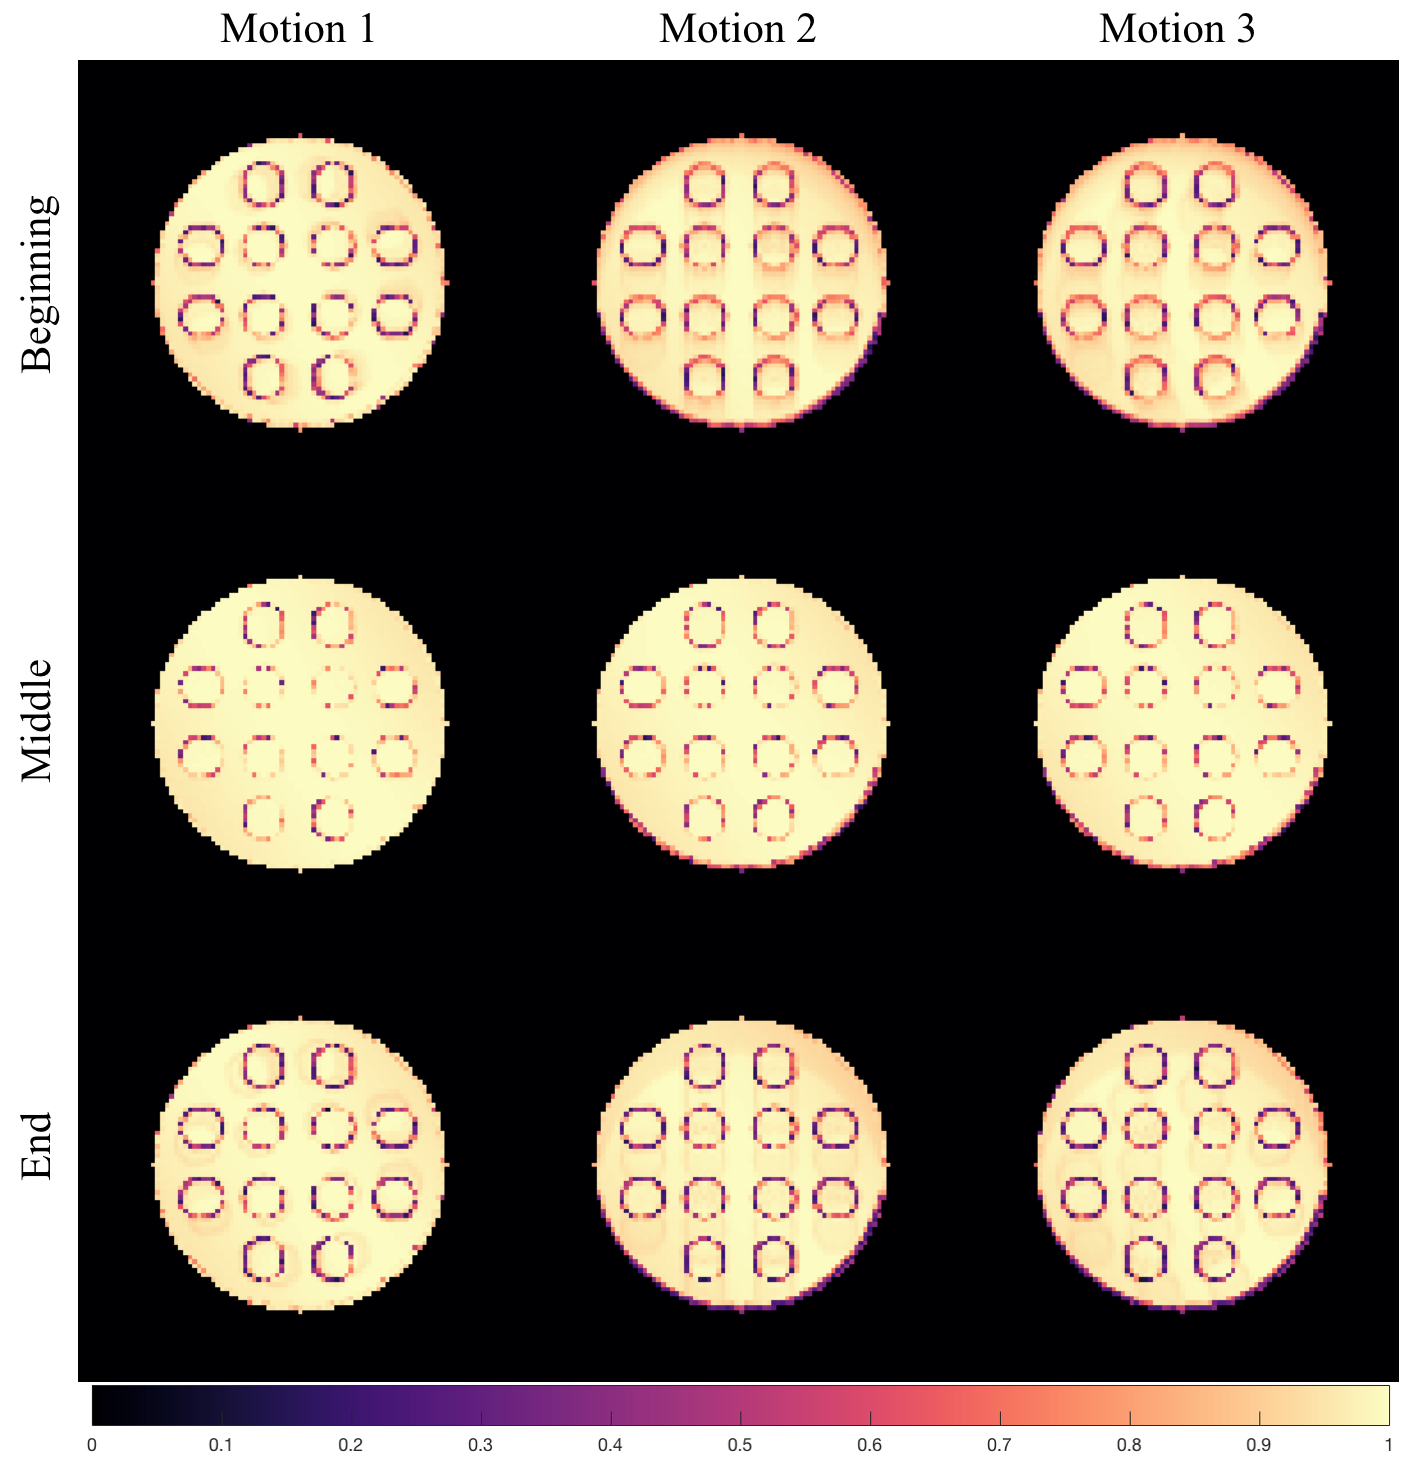
\includegraphics[width=1\textwidth]{images/mrf/scoremapsmotion}
    \caption{Motion corrupted matching score maps for all 9 types of motion traces. First column corresponds to the \textit{motion 1} trace (continuous rotation about the z-axis), the second column corresponds to the \textit{motion 2} trace (continuous translation along the y-axis) and the third column corresponds to the \textit{motion 3} trace (continuous rotation about the z-axis and continuous translation along the y-axis). Different lines correspond to a different onset of motion.}
    \label{fig:appendixscoremapsmotion}
\end{figure}

% T1 motion maps zoom
\begin{figure}[ht]
    \centering
    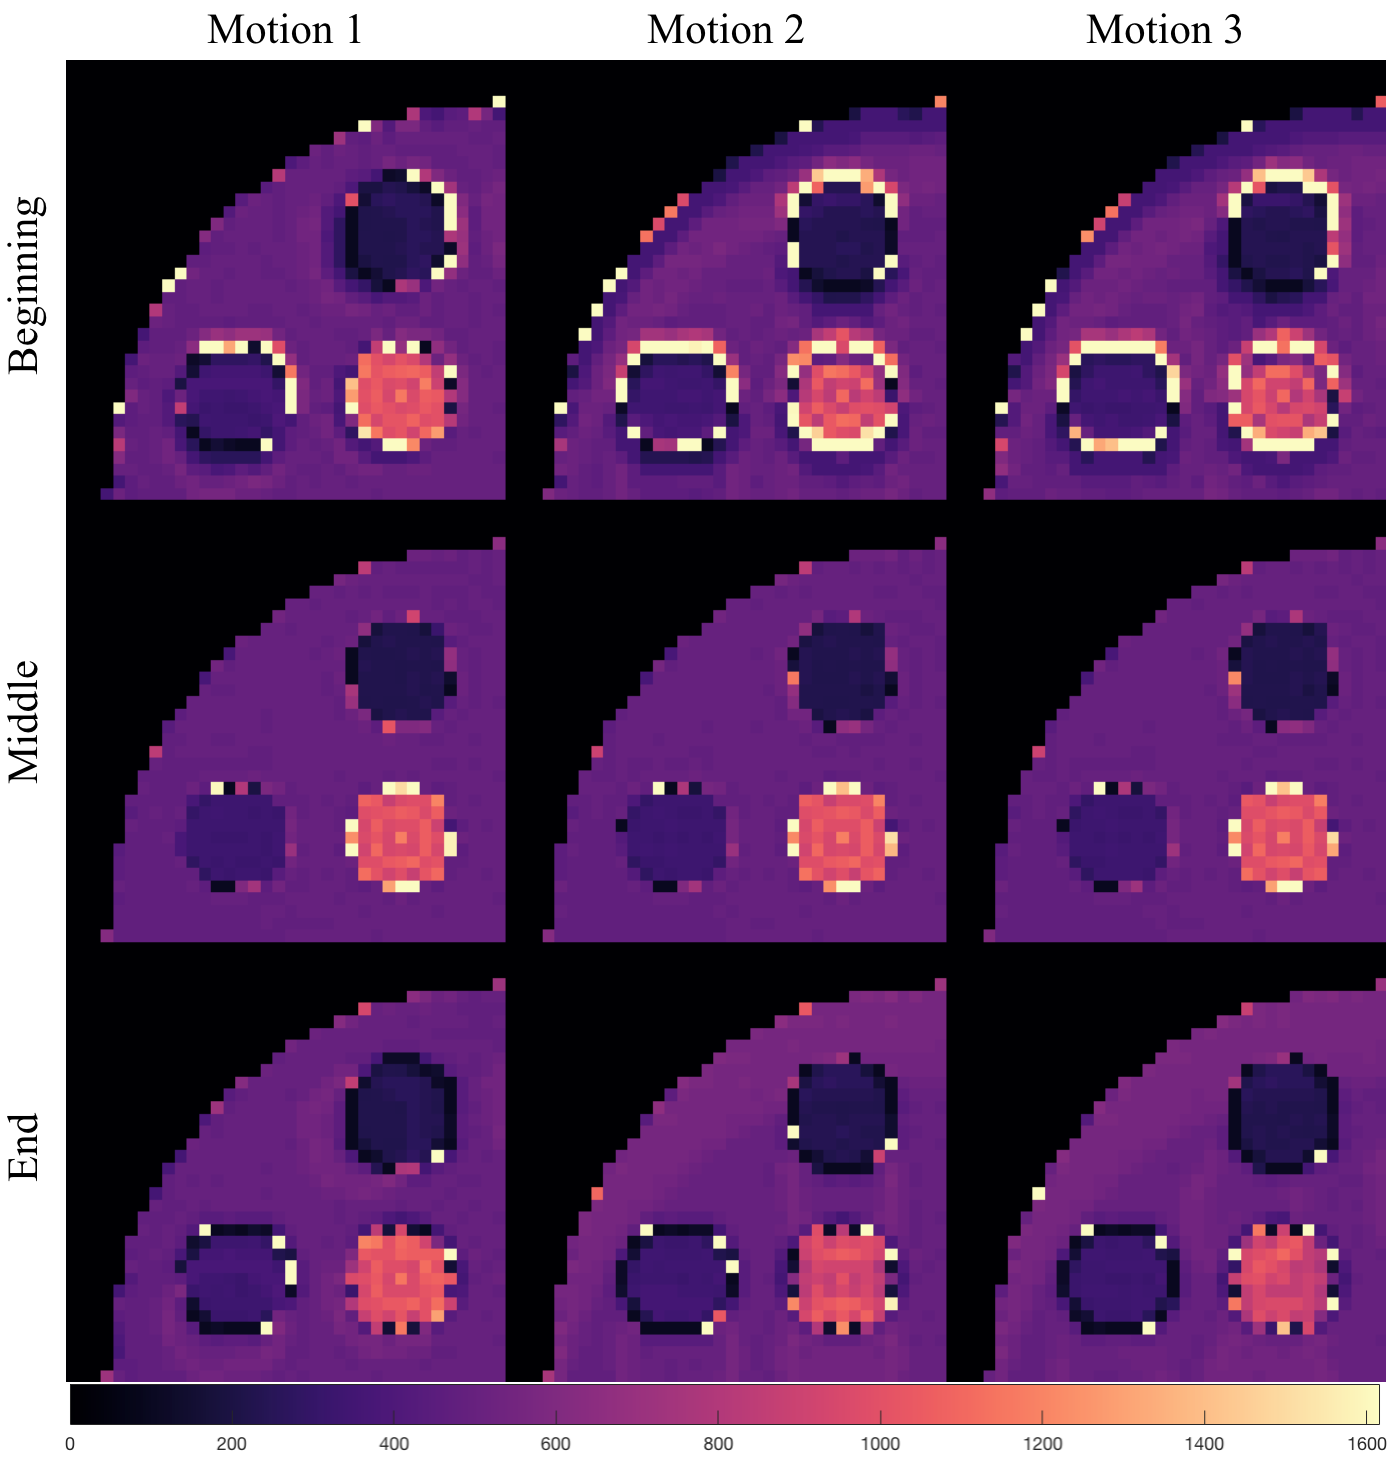
\includegraphics[width=1\textwidth]{images/mrf/T1mapsmotionzoom}
    \caption{Zoomed in $T_1$ maps for different types of motion}
    \label{fig:appendixT1mapsmotionzoom}
\end{figure}

% T2 motion maps zoom
\begin{figure}[ht]
    \centering
    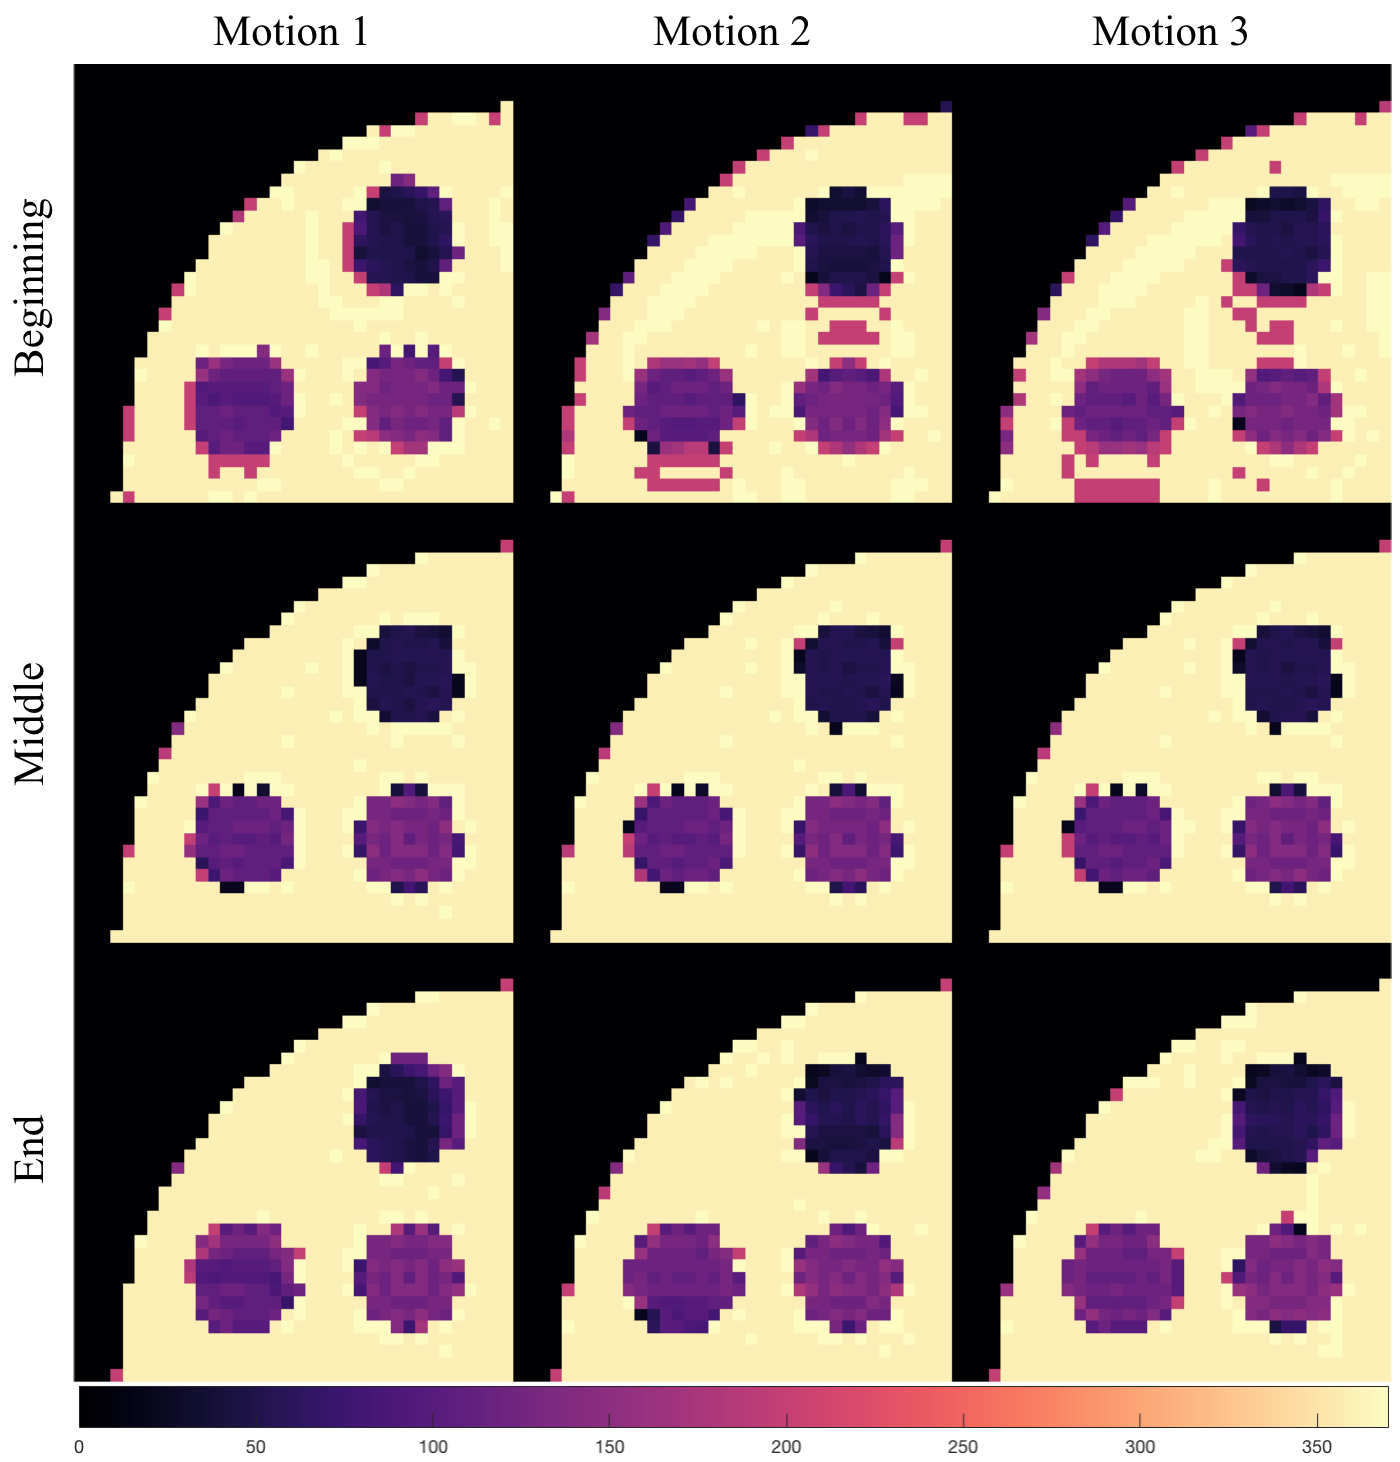
\includegraphics[width=1\textwidth]{images/mrf/T2mapsmotionzoom}
    \caption{Zoomed in $T_2$ maps for different types of motion}
    \label{fig:appendixT2mapsmotionzoom}
\end{figure}

% ROI analysis motion 1
\begin{figure}[ht]
    \makebox[\textwidth][c]{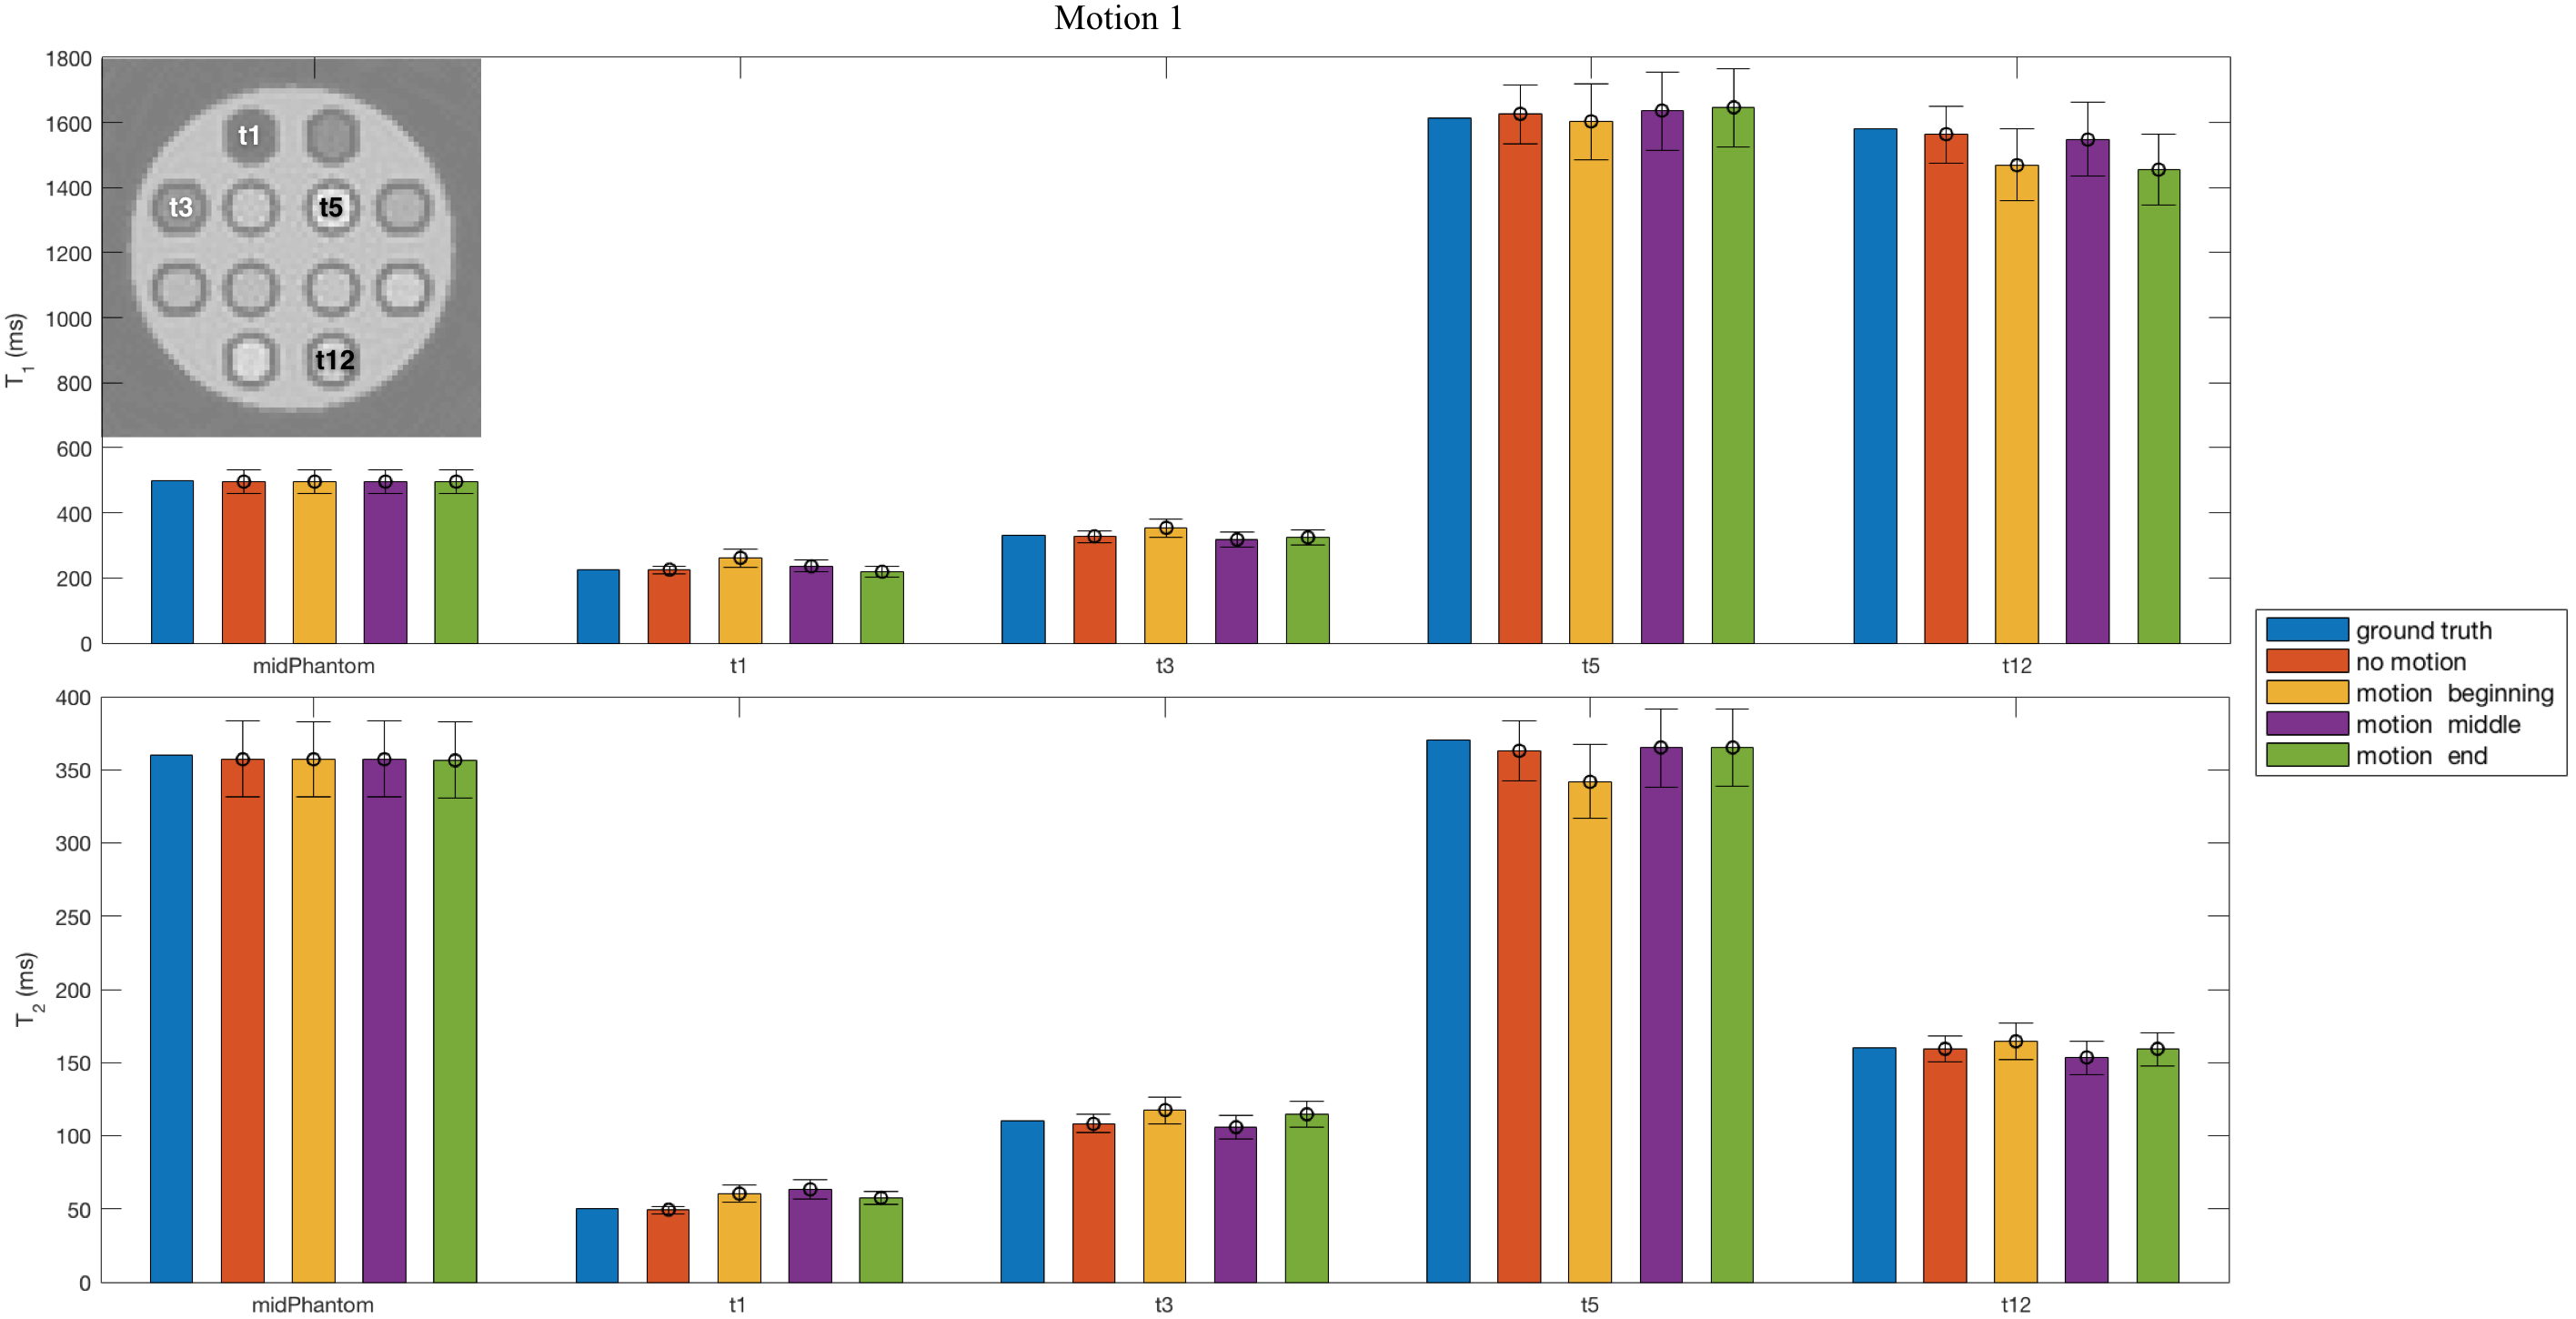
\includegraphics[width=1.4\textwidth]{images/mrf/motion1ROI}}
    \caption{Region of interest analysis on \textit{motion 1} for different motion onsets showing the average $T_1$ and $T_2$ values in 5 regions of the phantom.
    Different colours correspond to different onsets of motion, while different groups of bars correspond to a different part of the phantom, as shown in the upper left image.}
    \label{fig:appendixmotion1ROI}
\end{figure}

% ROI analysis motion 2
\begin{figure}[ht]
    \makebox[\textwidth][c]{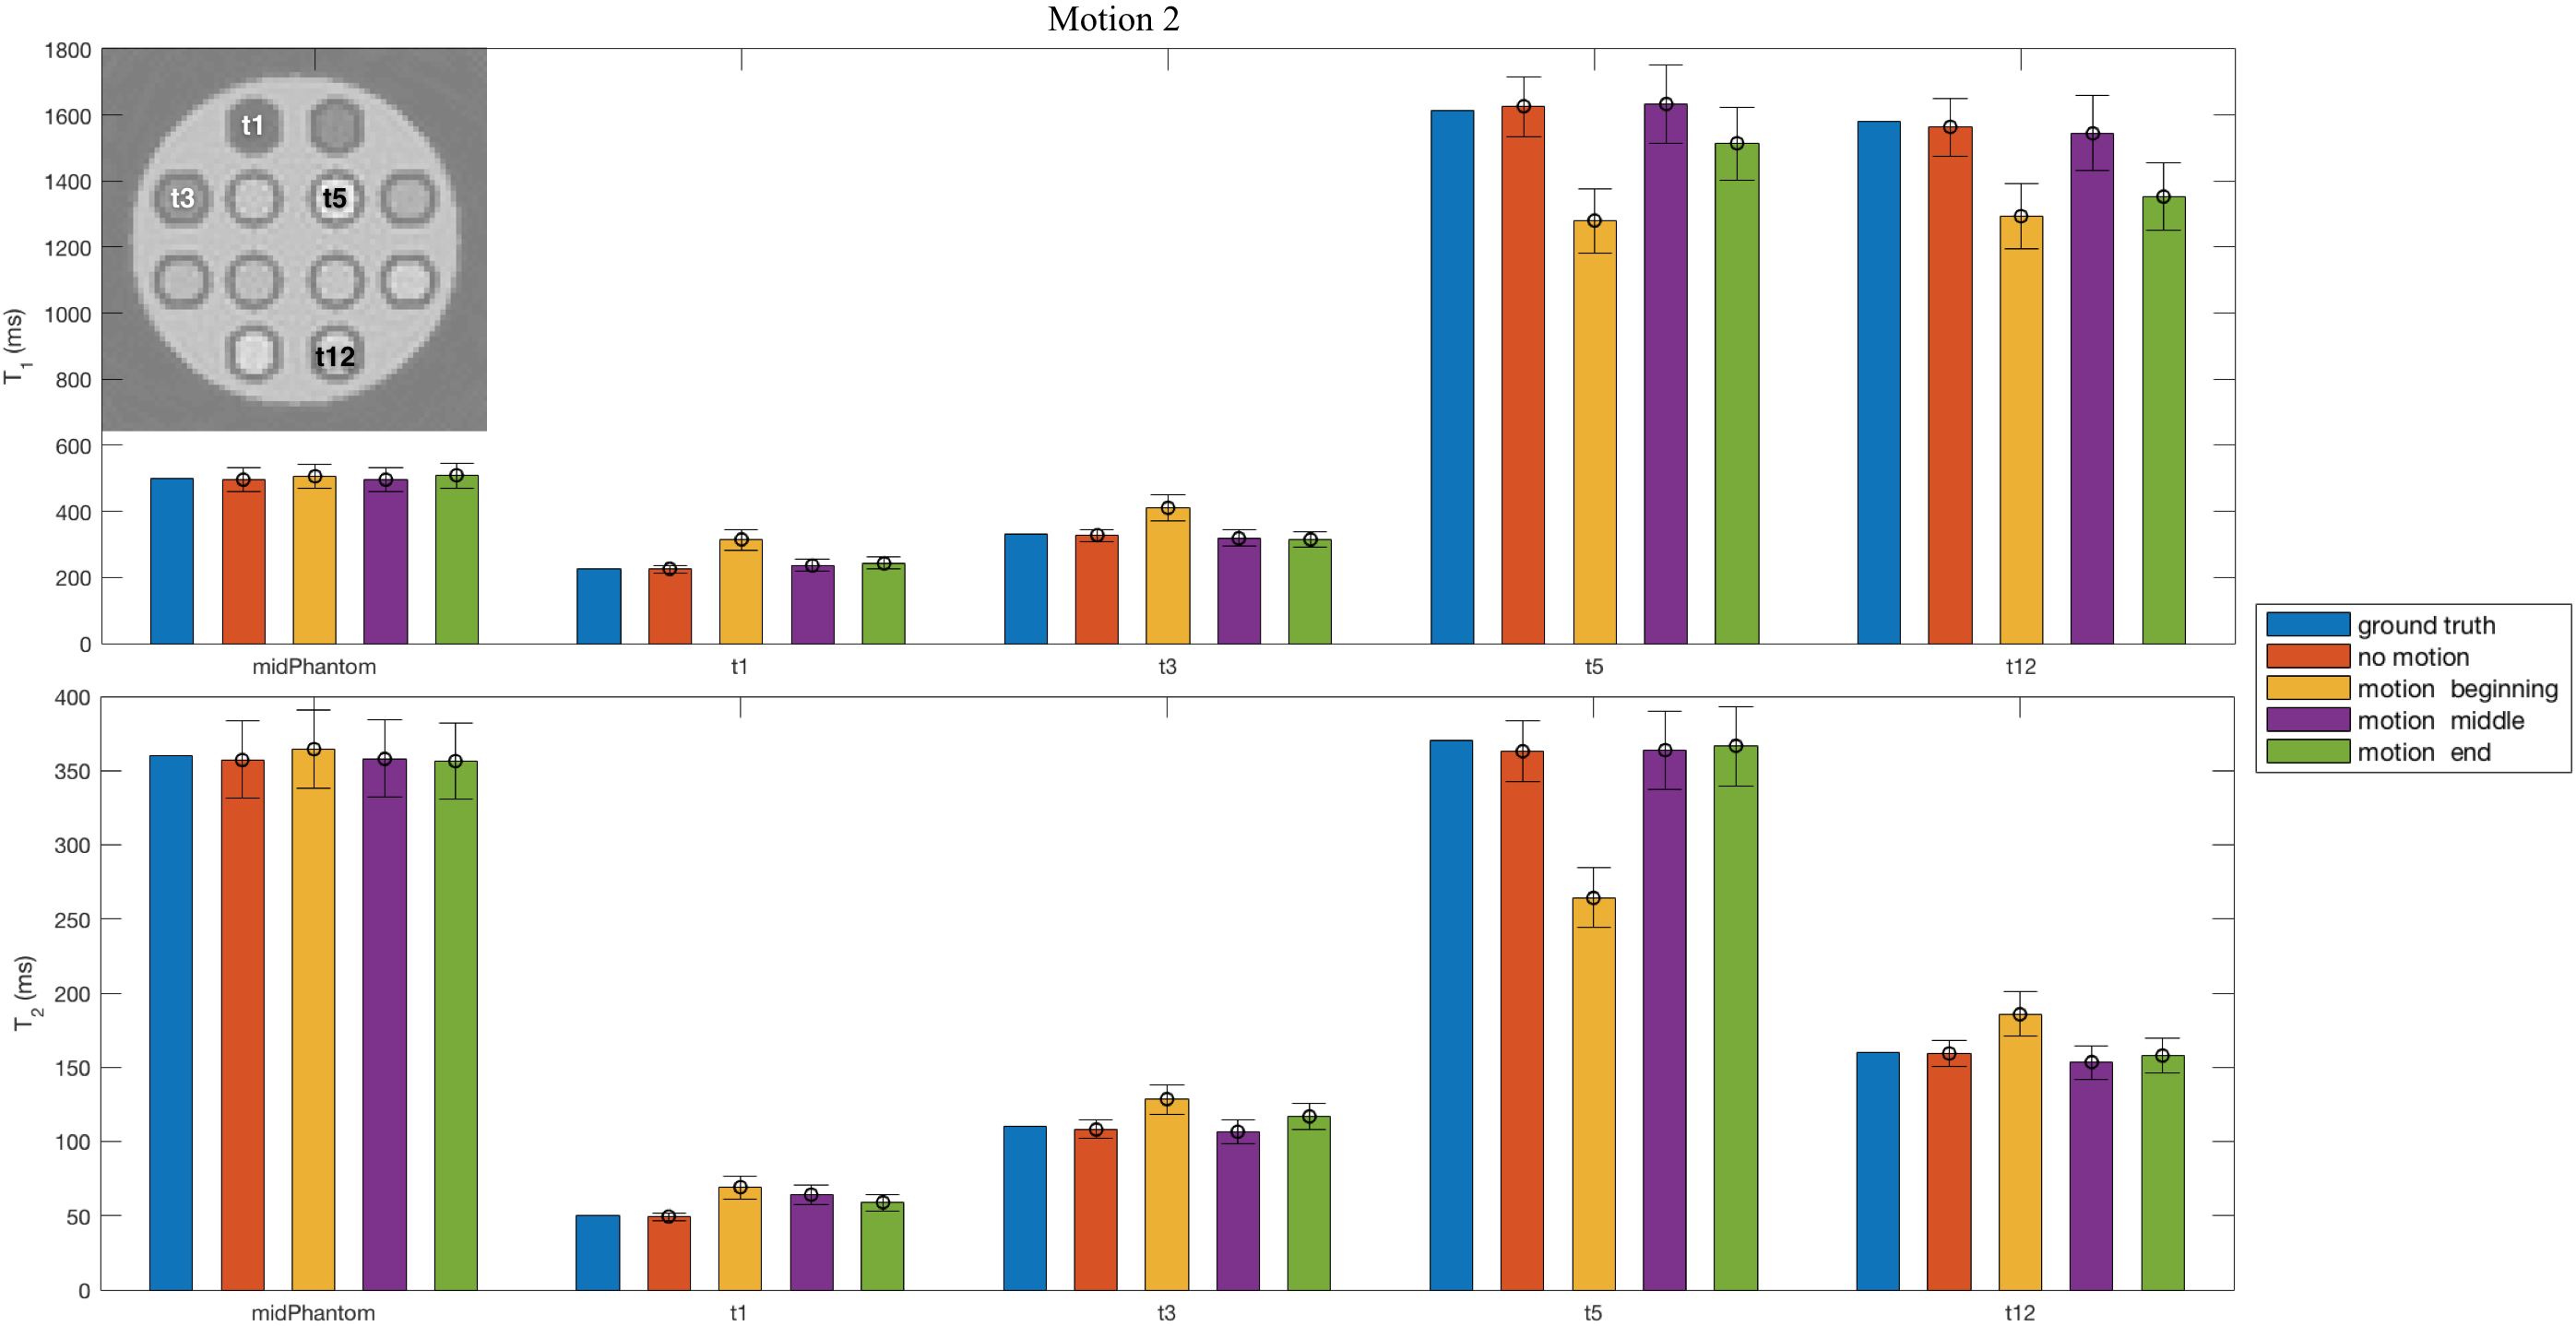
\includegraphics[width=1.4\textwidth]{images/mrf/motion2ROI}}
    \caption{Region of interest analysis on \textit{motion 2} for different motion onsets showing the average $T_1$ and $T_2$ values in 5 regions of the phantom..
    Different colours correspond to different onsets of motion, while different groups of bars correspond to a different part of the phantom, as shown in the upper left image.}
    \label{fig:appendixmotion2ROI}
\end{figure}

% ROI analysis motion 3
\begin{figure}[ht]
    \makebox[\textwidth][c]{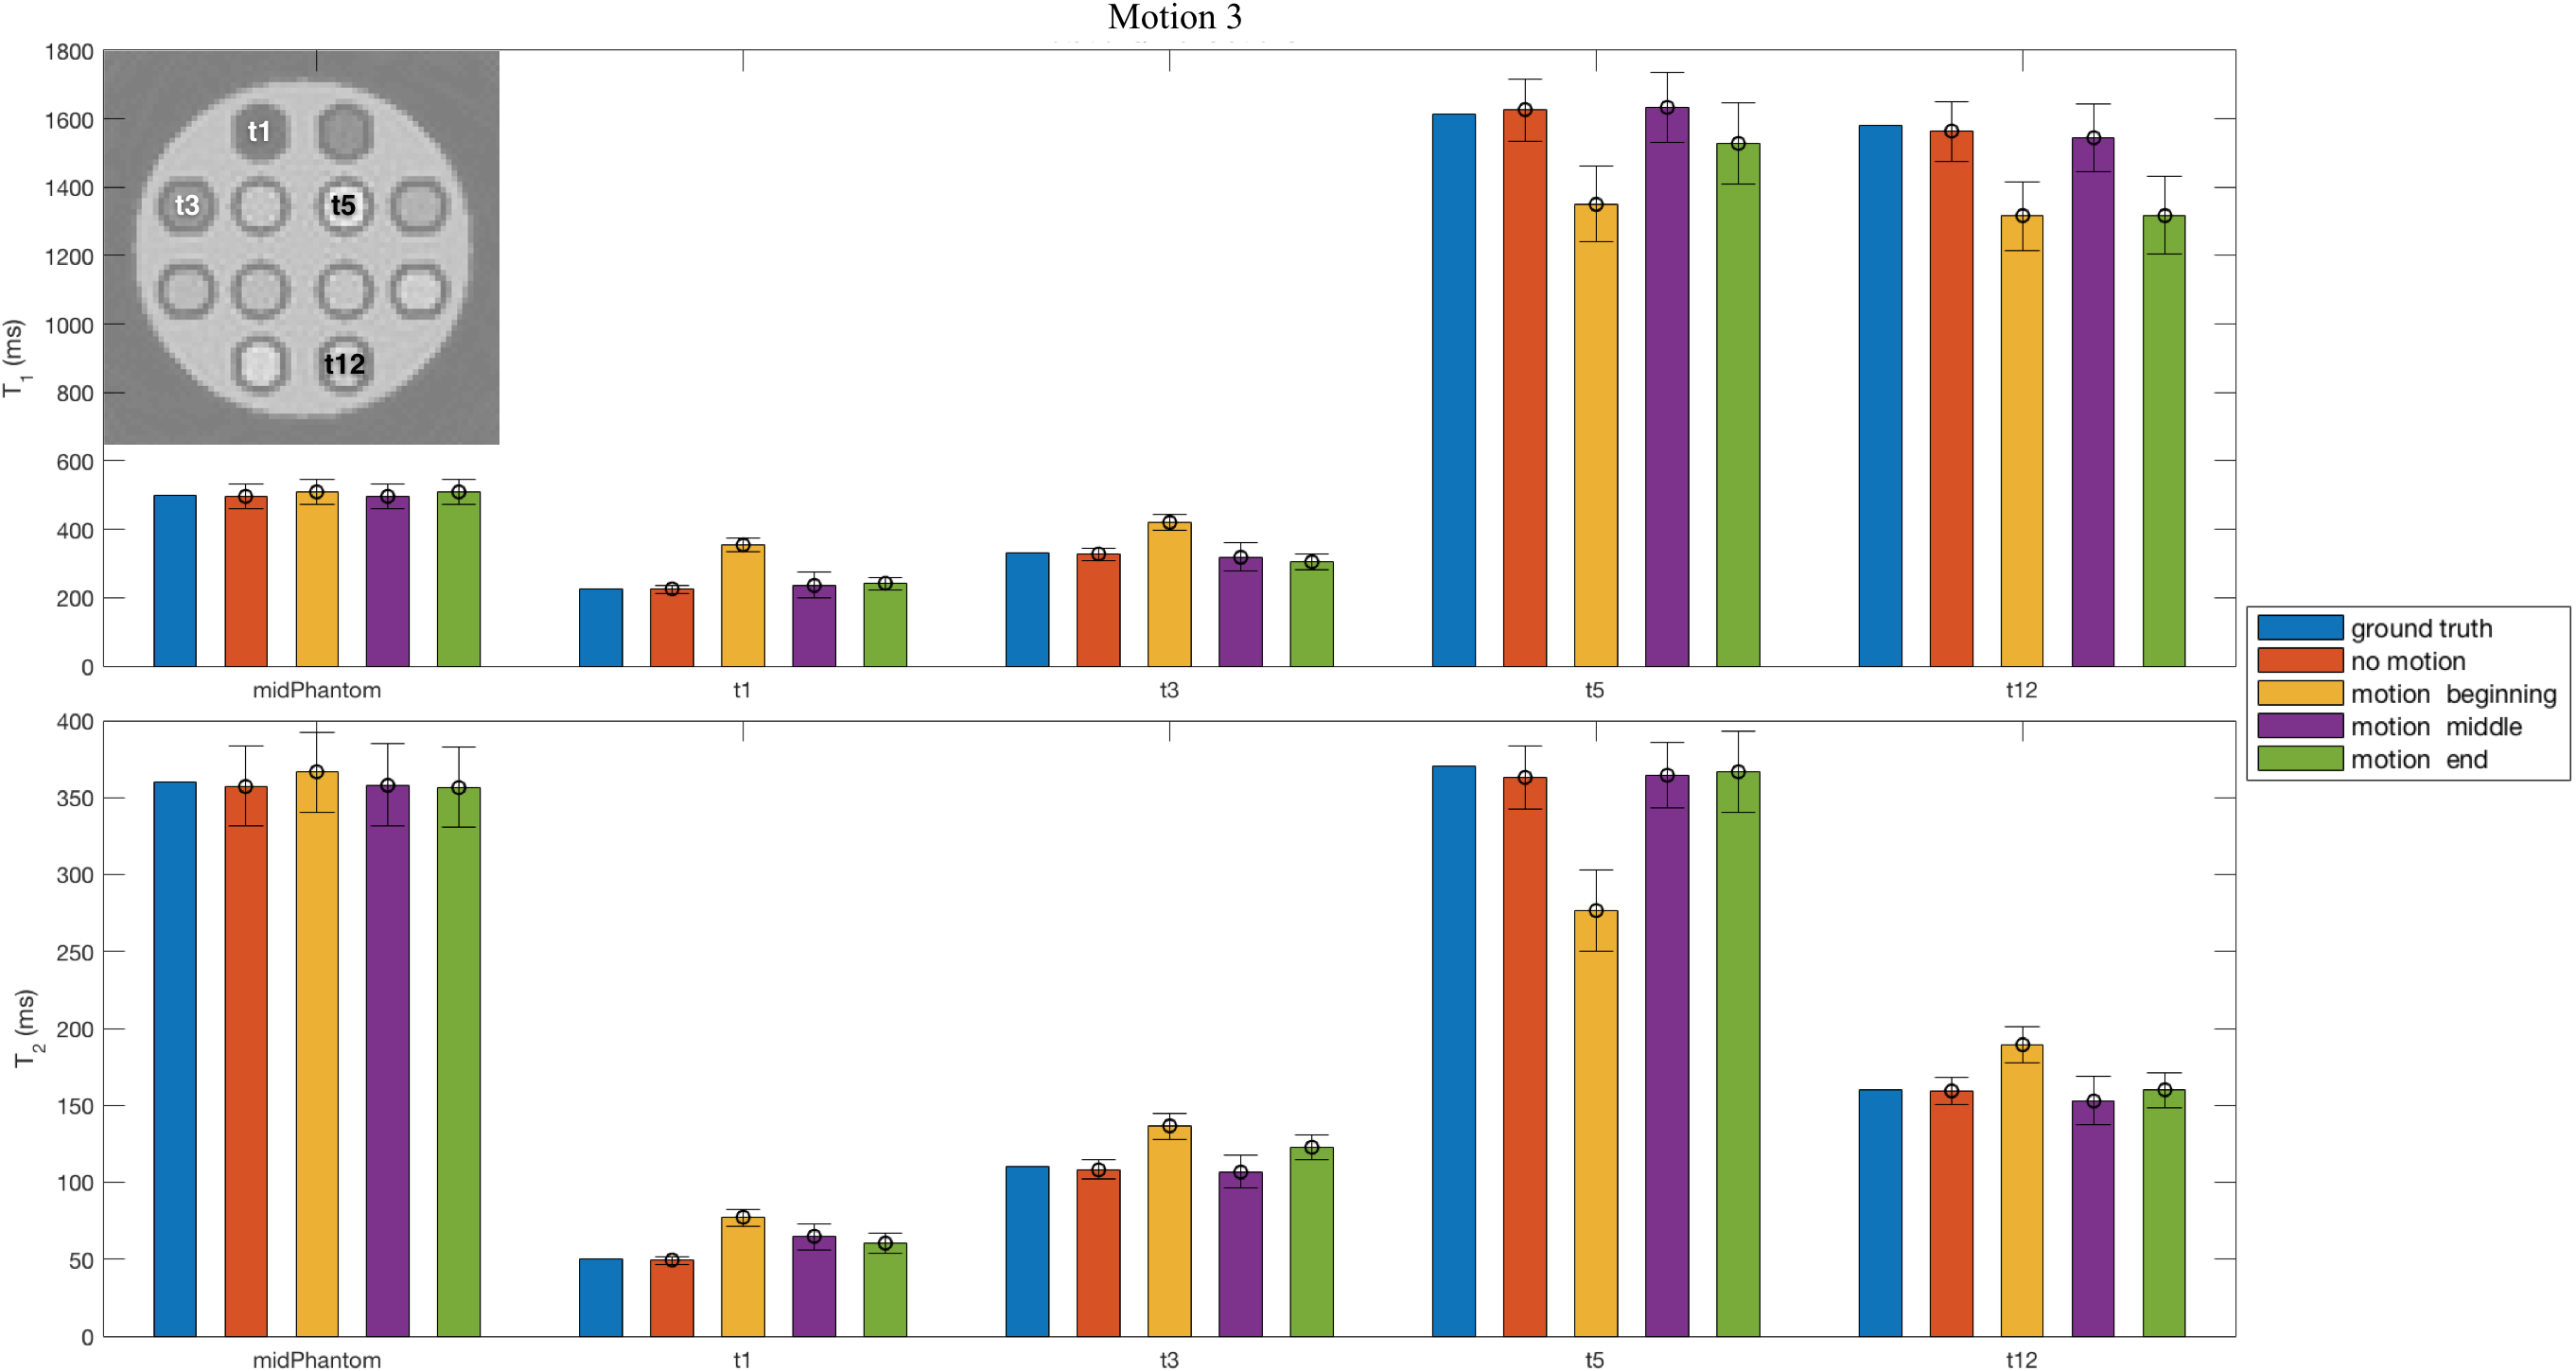
\includegraphics[width=1.4\textwidth]{images/mrf/motion3ROI}}
    \caption{Region of interest analysis on \textit{motion 3} for different motion onsets showing the average $T_1$ and $T_2$ values in 5 regions of the phantom.
    Different colours correspond to different onsets of motion, while different groups of bars correspond to a different part of the phantom, as shown in the upper left image.}
    \label{fig:appendixmotion3ROI}
\end{figure}